\documentclass[11pt]{article}

\usepackage[utf8]{inputenc}
\usepackage[T1]{fontenc}
\usepackage{lmodern}
\usepackage[a4paper,margin=0.88in]{geometry}
\usepackage{amsmath,amssymb,amsthm,mathtools}
\usepackage{xcolor}
\usepackage[most]{tcolorbox}
\usepackage{booktabs,array,tabularx}
\usepackage{enumitem}
\usepackage{titlesec}
\usepackage{parskip}
\usepackage{tikz}
\usetikzlibrary{arrows.meta,positioning,fit,calc}
\usepackage[colorlinks=true,linkcolor=blue!55!black,urlcolor=blue!60!black,citecolor=blue!55!black]{hyperref}

\definecolor{accent}{HTML}{006D77}
\definecolor{accent2}{HTML}{2F6B3C}
\definecolor{accent3}{HTML}{B45309}
\definecolor{soft}{HTML}{EAF6F7}
\definecolor{cool}{HTML}{ECF7ED}
\definecolor{warm}{HTML}{FFF4E6}
\definecolor{risk}{HTML}{A61B1B}

\titleformat{\section}{\Large\bfseries\color{accent}}{\thesection}{0.55em}{}
\titleformat{\subsection}{\large\bfseries\color{accent!85!black}}{\thesubsection}{0.55em}{}
\titlespacing*{\section}{0pt}{1.4em}{0.5em}

\newtcolorbox{keybox}[1][]{colback=soft,colframe=accent,boxrule=.7pt,arc=2pt,
  left=7pt,right=7pt,top=5pt,bottom=5pt,fonttitle=\bfseries,#1}
\newtcolorbox{theorybox}[1][]{colback=cool,colframe=accent2,boxrule=.7pt,arc=2pt,
  left=7pt,right=7pt,top=5pt,bottom=5pt,fonttitle=\bfseries,title={Theory target},#1}
\newtcolorbox{riskbox}[1][]{colback=red!3,colframe=risk,boxrule=.7pt,arc=2pt,
  left=7pt,right=7pt,top=5pt,bottom=5pt,fonttitle=\bfseries,title={Falsification gate},#1}
\newtcolorbox{claimbox}[1][]{colback=warm,colframe=accent3,boxrule=.8pt,arc=2pt,
  left=7pt,right=7pt,top=5pt,bottom=5pt,fonttitle=\bfseries,title={Claim allowed only if the experiments support it},#1}

\newtheorem{proposition}{Proposition}
\newtheorem{targettheorem}{Target theorem}

\newcommand{\R}{\mathbb{R}}
\newcommand{\E}{\mathbb{E}}
\newcommand{\norm}[1]{\left\lVert #1\right\rVert}
\newcommand{\softmax}{\operatorname{softmax}}
\newcommand{\bytes}{\operatorname{Bytes}}
\newcommand{\cost}{\operatorname{Cost}}
\newcommand{\term}[1]{\textbf{\color{accent!85!black}#1}}

\begin{document}
\pagenumbering{roman}

\begin{titlepage}
\centering
\vspace*{1.25cm}
{\Huge\bfseries\color{accent} CP-Direct-KV\par}
\vspace{0.25cm}
{\Large\bfseries Reconstruction-Free CP-Decomposed\ KV Attention on a Single Device\par}
\vspace{0.45cm}
{\large Born-compressed coefficients, bounded SVD-free adaptation,\ RoPE-pair-aligned residuals, and GEMM-friendly kernels\par}
\vspace{1.0cm}
\begin{tcolorbox}[colback=soft,colframe=accent,width=.94\textwidth,arc=3pt]
\centering\bfseries
CP-Direct-KV represents old layer-wise KV tensors with CANDECOMP/PARAFAC factors and derives
attention algebra that reads those factors directly. Its goal is a practical tensor method whose
runtime is dominated by regular matrix operations rather than dense-cache reconstruction.
\end{tcolorbox}
\vspace{.7cm}
\begin{tcolorbox}[colback=warm,colframe=accent3,width=.94\textwidth,arc=3pt]
\small
\textbf{Positioning.} This is a \emph{Technique Paper} and the lower-risk companion to CATT-KV.
CP is not claimed as a new decomposition. The proposed contributions are the CP layout selected for
KV semantics, exact reconstruction-free attention algebra, a two-mode encode/adapt lifecycle, and a
latency-aware rank/residual policy validated against low-bit quantization.
\end{tcolorbox}
\vfill
{\normalsize Rigorous research proposal \;\textbullet\; July 2026\par}
\end{titlepage}

\tableofcontents
\newpage
\pagenumbering{arabic}

\section{Executive decision}

\begin{keybox}[title={One-sentence key idea}]
Factor each old KV block over token, KV-head, RoPE-pair, and pair-component modes, cache the CP token
coefficients and small global/block factors, and evaluate logits and value aggregation by GEMMs over
the factors without reconstructing a token's full K or V vector.
\end{keybox}

CP-Direct-KV trades some of CATT-KV's multiscale expressiveness for simpler execution. Its direct
attention equations reduce to dense, contiguous matrix products; therefore it has a more credible
path to speedup on Jetson and standard NVIDIA GPUs. Its scientific risk is instead representational:
CP can be ill-conditioned, its best low-rank approximation may be unstable, and a shared token
factor may require too high a rank on heterogeneous heads. Regularization and explicit stop gates
are therefore part of the proposal.

\begin{center}
\small
\renewcommand{\arraystretch}{1.22}
\begin{tabularx}{.98\textwidth}{@{}p{2.55cm}X p{2.2cm}@{}}
\toprule
\textbf{Axis} & \textbf{Required contribution} & \textbf{Gate} \\
\midrule
Representation & CP over token/head/RoPE-pair/component with separate K and V factors & $\ge 4\times$ physical KV reduction \\
Online cost & Fixed-factor encoding or at most two block CP-ALS sweeps & Positive payback within 128 future queries \\
Execution & Direct logits and V aggregation through factors & No $B\times H\times d$ old-cache allocation \\
Quality & Attention-weighted fitting plus pair-block sparse innovations & Near-full-cache task quality at selected budget \\
Competitiveness & Same-byte comparison with INT4 and modern tensor/matrix baselines & Better latency or quality at matched memory \\
\bottomrule
\end{tabularx}
\end{center}

\section{Research gap and novelty boundary}

Existing low-rank KV methods mostly use matrices: Palu factorizes projection weights and caches a
latent state~\cite{palu}; Eigen Attention computes in a reduced subspace~\cite{eigen}; OjaKV adapts
a matrix basis online~\cite{ojakv}; and RAP prunes RoPE-aligned coordinate pairs to avoid
reconstruction~\cite{rap}. Tensor methods include MPO-based DecoQuant~\cite{decoquant} and partial
Tucker plus residual allocation in JoLT~\cite{jolt}. Sparse dictionaries also reconstruct KV from
selected atoms~\cite{lexico}.

CP-Direct-KV occupies a narrower space: it uses a CP model whose factors correspond to the semantic
modes of the physical cache and rewrites both sides of attention in factor form. A July 2026 search
did not find a prior KV method with this exact CP execution path; that search is evidence for a
novelty hypothesis, not proof. A final submission must repeat the search across arXiv, OpenReview,
DBLP, Semantic Scholar, and patent databases.

\begin{center}
\scriptsize
\renewcommand{\arraystretch}{1.22}
\begin{tabularx}{\textwidth}{@{}p{2.0cm}p{2.25cm}p{2.25cm}p{2.25cm}X@{}}
\toprule
\textbf{Family} & \textbf{Factorization target} & \textbf{Runtime adaptation} & \textbf{Attention path} & \textbf{Difference} \\
\midrule
Palu / Eigen & Feature matrix & None / calibration & Reduced projection or reconstruction & No head--pair CP structure \\
OjaKV & Per-cache matrix basis & Online PCA-style & Reconstructed approximate KV & Matrix update; no CP factor algebra \\
DecoQuant & Matrix reshaped as MPO & Data-free & Dequantization kernel & Tensorization primarily improves quantization \\
JoLT & Token/feature Tucker & Block decomposition & Compressed storage focus & Tucker plus randomized-SVD variant \\
Lexico & Sparse dictionary & Per-token coding & Sparse KV reconstruction & Does not compute softmax attention in factor space \\
\textbf{CP-Direct-KV} & Token, head, pair, component CP & Encode-only or bounded block ALS & \textbf{Direct factor GEMMs} & Joint semantic modes, pair residual, payback gate \\
\bottomrule
\end{tabularx}
\end{center}

\begin{claimbox}
Do not claim ``the first tensor KV cache.'' Claim a CP-specific representation/execution co-design
only after confirming the novelty search and demonstrating that direct factor attention, rather
than CP storage alone, changes the end-to-end Pareto frontier.
\end{claimbox}

\section{Thinking template and logic chain}

\small
\renewcommand{\arraystretch}{1.18}
\begin{tabularx}{\textwidth}{@{}p{3.35cm}X@{}}
\toprule
\textbf{Stage} & \textbf{Proposal content} \\
\midrule
Research background & Long-context inference is memory-bandwidth bound because every decoded token
reads all prior K/V. Low-rank and tensor compression help only when their representation can be
created and consumed more cheaply than the dense cache. \\
Limitation 1 & Matrix projections discard multiway head/frequency structure; existing tensor methods
do not expose a CP attention algebra optimized for regular GEMMs. \\
Limitation 2 & A purely offline factor basis is brittle under prompt shift, while unconstrained
runtime CP-ALS is too expensive and may be unstable. \\
Limitation 3 & CP reconstruction error alone does not protect softmax routing, and arbitrary sparse
residuals can destroy kernel regularity. \\
Key idea & Use a semantic CP cache that is born as token coefficients or adapted once per aged block,
then consumed directly with RoPE-pair-aligned sparse corrections. \\
Challenge 1 & Choose CP modes and rank so factors compress both GQA and MHA caches without forcing
unrelated K/V structure. \\
Challenge 2 & Bound runtime fitting and make both attention phases factor-executable. \\
Challenge 3 & Correct attention-critical approximation failures without irregular scalar sparsity. \\
Module A & Separate K/V semantic CP with encode-only and bounded-adapt modes. \\
Module B & Direct CP logits/value kernels plus payback-aware rank control. \\
Module C & Query-weighted fitting, RoPE-pair block residuals, and attention-error guarantees. \\
Contributions & C1 CP cache representation (Sec.~\ref{sec:cp}); C2 reconstruction-free equations and
kernels (Sec.~\ref{sec:direct}); C3 bounded adaptation, residual, and analysis
(Secs.~\ref{sec:lifecycle}--\ref{sec:theory}); C4 end-to-end evaluation
(Sec.~\ref{sec:experiments}). \\
\bottomrule
\end{tabularx}
\normalsize

The four consistency checks pass. The representation module answers the missing multiway layout;
the lifecycle/direct-kernel module answers runtime feasibility; the structured-residual module
answers routing risk. Each claimed contribution is backed by a named method or experiment section.

\section{Formal problem and CP representation}
\label{sec:cp}

For a layer and closed token block, reshape the K cache as
\[
\mathcal K\in\R^{B\times H\times P\times 2}, \qquad P=d/2,
\]
where the final mode preserves the two coordinates of each RoPE pair. Use separate rank-$R_K$ and
rank-$R_V$ CP models:
\begin{align}
\widehat{\mathcal K}_{shpu}
&=\sum_{r=1}^{R_K}A^K_{sr}B^K_{hr}C^K_{pr}D^K_{ur}, \label{eq:cpk}\\
\widehat{\mathcal V}_{shpu}
&=\sum_{r=1}^{R_V}A^V_{sr}B^V_{hr}C^V_{pr}D^V_{ur}. \label{eq:cpv}
\end{align}
Here $s$ is token, $h$ is KV head, $p$ is RoPE/frequency pair, and $u\in\{0,1\}$ is the pair
component. K and V never share factors by default; shared factors are an ablation because the two
objects play different roles and have different compressibility.

\begin{proposition}[CP storage]
The scalar count for one K block is
$R_K(B+H+P+2)$ instead of $2BHP$; V is analogous. The paper reports physical bytes after padding,
factor scales, residual indices, and alignment.
\end{proposition}

For GQA, $H$ may be small enough that a separate CP per head is competitive. Therefore evaluate two
layouts: \term{joint-head CP} as above and \term{head-private CP},
$\mathcal K_h\in\R^{B\times P\times2}$. The controller chooses by measured bytes and latency, not
by an assumption that joint factorization is always better.

\section{Two-mode cache lifecycle}
\label{sec:lifecycle}

\subsection{Mode E: encode-only, born compressed}

Offline calibration learns layer-specific non-token atoms
$\Phi_r=B_{:r}\circ C_{:r}\circ D_{:r}$. For each generated full K or V token tensor $x_s$, compute
only its coefficient vector
\[
a_s=(\Phi^\top\Phi+\gamma I)^{-1}\Phi^\top\operatorname{vec}(x_s),
\]
using a precomputed regularized Gram inverse, append $a_s$ to $A$, then release $x_s$. This path is
SVD-free and makes cache growth $R$ rather than $2HP$ scalars per token. Training the atoms uses a
calibration corpus and an attention-distillation loss; the base LLM weights remain frozen.

\subsection{Mode A: bounded block adaptation}

Encode-only factors may fail under domain shift. In adaptive mode, keep a native exact hot block.
When it ages, initialize CP from the calibrated atoms and run at most $J\in\{1,2\}$ regularized
CP-ALS sweeps. Each sweep is implemented through MTTKRP and small Gram solves; no SVD is permitted.
Randomized CP-ALS sampling is a fallback for large blocks~\cite{randcp}. Factors are normalized each
sweep, component weights are clipped, and nearly collinear components are merged or pruned to
limit degeneracy.

The runtime selects Mode E, Mode A, INT4, or native storage from a per-layer cost table. Mode A is
admitted only if measured fit cost can be recovered over the predicted remaining queries.

\begin{keybox}[title={Why both modes belong in one paper}]
They share the same CP cache and direct kernels. Mode E tests the lowest-overhead deployment point;
Mode A tests whether a tiny amount of prompt adaptation buys enough quality to justify its cost.
The paper does not propose a general CP optimizer; it proposes a bounded KV lifecycle.
\end{keybox}

\section{Reconstruction-free CP attention}
\label{sec:direct}

Let a query for KV head $h$ be $q_h\in\R^{P\times2}$. Define
\[
g^K_{hr}(q)=B^K_{hr}\sum_{p=1}^{P}\sum_{u=0}^{1}
q_{hpu}C^K_{pr}D^K_{ur}.
\]
Then the score for all $B$ tokens is
\begin{equation}
\widehat s_h=A^K g^K_h(q)/\sqrt d. \label{eq:logits}
\end{equation}
Equation~\eqref{eq:logits} is a matrix-vector product; it never constructs
$\widehat{\mathcal K}_{s,h,:,:}$. After online softmax gives $\alpha_h\in\R^B$, define
\[
z^V_{hr}=\sum_{s=1}^{B}\alpha_{hs}A^V_{sr}.
\]
The attention output is
\begin{equation}
\widehat o_{hpu}=\sum_{r=1}^{R_V}z^V_{hr}B^V_{hr}C^V_{pr}D^V_{ur}. \label{eq:value}
\end{equation}
This is again a short GEMM followed by factor scaling. Equations~\eqref{eq:logits} and
\eqref{eq:value} are algebraically exact for the approximate CP cache.

\begin{proposition}[Direct-execution complexity]
For one head and block, CP logits require $O(R_Kd+BR_K)$ operations and CP value aggregation
requires $O(BR_V+R_Vd)$, versus $O(Bd)$ for each dense phase. CP reduces bytes read when
$R\ll d$, but arithmetic is lower only in a rank-dependent region that must be measured.
\end{proposition}

The implementation fuses factor scaling, GEMM, sparse residual contributions, and online softmax.
The exact hot block and all old CP blocks contribute partial softmax maxima, denominators, and
numerators, which are merged with the standard numerically stable block-softmax identity.

\begin{center}
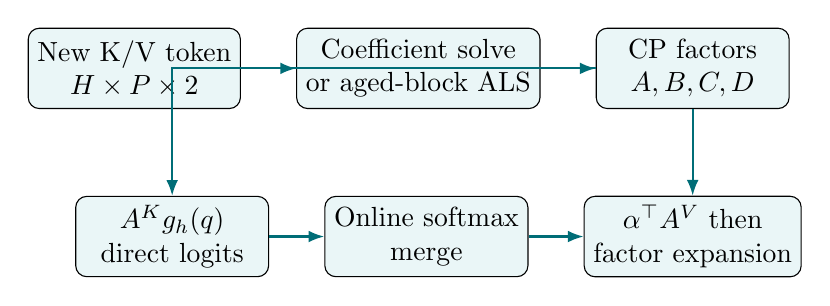
\begin{tikzpicture}[
  box/.style={draw,rounded corners,minimum height=1.02cm,minimum width=2.45cm,align=center,fill=soft},
  arr/.style={-{Latex[length=2mm]},thick,accent}]
\node[box] (kv) {New K/V token\\$H\times P\times2$};
\node[box,right=7mm of kv] (enc) {Coefficient solve\\or aged-block ALS};
\node[box,right=7mm of enc] (fac) {CP factors\\$A,B,C,D$};
\node[box,below=11mm of fac] (v) {$\alpha^\top A^V$ then\\factor expansion};
\node[box,left=7mm of v] (sm) {Online softmax\\merge};
\node[box,left=7mm of sm] (k) {$A^Kg_h(q)$\\direct logits};
\draw[arr] (kv)--(enc); \draw[arr] (enc)--(fac);
\draw[arr] (fac)--(v); \draw[arr] (fac.west) -| (k.north);
\draw[arr] (k)--(sm); \draw[arr] (sm)--(v);
\end{tikzpicture}
\end{center}

\section{RoPE handling and structured sparse residual}

CP-Direct-KV initially factorizes \emph{post-RoPE} keys. This keeps Equation~\eqref{eq:logits}
simple and correct but may raise CP rank because rotation couples token position and frequency pair.
The pair mode is retained explicitly so the method can measure and correct that effect rather than
hiding it in a flattened feature axis.

Two RoPE variants are evaluated:
\begin{enumerate}[leftmargin=1.55em,itemsep=2pt]
\item \term{Post-RoPE CP}: factorize the cache exactly as consumed by ordinary attention; simplest
and primary implementation.
\item \term{Phase-augmented CP}: add analytic sine/cosine-modulated token factors for selected
frequency bands. This increases factor count but may reduce base CP rank. It is an ablation, not a
required contribution, because RAP and frequency-aware methods already make generic RoPE claims
novelty-sensitive~\cite{rap}.
\end{enumerate}

Let $e^K_{shp:}=K_{shp:}-\widehat K_{shp:}$ and similarly for V. The residual unit is an entire
two-coordinate RoPE pair. Pair score
\[
I_{shp}=\max_{q\in\mathcal Q}|q_{hp:}^{\top}e^K_{shp:}|
+\eta\bar\alpha_{hs}\norm{e^V_{shp:}}_2
\]
selects the top $k$ pair blocks. This avoids scalar index scatter, preserves pair rotation, and
targets errors capable of changing attention rather than merely the largest tensor entries.

\section{Attention-aware fitting and controller}

Calibration and bounded adaptation minimize
\begin{align}
L=&\;\E_{(K,V,Q)}\left[
\norm{\softmax(QK^\top/\sqrt d)V-
\softmax(Q\widehat K^\top/\sqrt d)\widehat V}_F^2\right] \\
&+\lambda_K\norm{K-\widehat K}_{W_K}^2
+\lambda_V\norm{V-\widehat V}_{W_V}^2
+\gamma\sum_r\left(\norm{B_{:r}}_2^2+\norm{C_{:r}}_2^2+\norm{D_{:r}}_2^2\right),
\end{align}
where weighted reconstruction supplies a cheap ALS-compatible surrogate and attention distillation
is evaluated periodically. Runtime Mode A uses the surrogate plus one final attention-error check;
it does not backpropagate through long sequences during decoding.

For each layer/head layout, the controller solves a small profiled choice:
\[
\min_{m\in\{\text{native, INT4, E, A}\},R,k}
\widehat L_{\rm attn}+\lambda M+\mu T_{\rm query}+\nu T_{\rm fit}
\]
subject to memory and expected-payback constraints. Rank is searched over a small discrete set; no
claim of solving CP rank globally is made.

\section{Theory targets}
\label{sec:theory}

\begin{targettheorem}[Direct CP attention equivalence]
Prove Equations~\eqref{eq:logits}--\eqref{eq:value} equal standard softmax attention evaluated on
the reconstructed CP tensors, up to floating-point order, while requiring no reconstructed KV
allocation. Extend the proof to stable block-softmax merging and sparse pair corrections.
\end{targettheorem}

\begin{targettheorem}[One-query output error]
For $\epsilon_K=\max_s\norm{K_s-\widehat K_s}_2$,
$\epsilon_V=\max_s\norm{V_s-\widehat V_s}_2$, and bounded approximate values, establish
\[
\norm{o(q)-\widehat o(q)}_2
\le \epsilon_V+2V_{\max}\norm q_2\epsilon_K/\sqrt d,
\]
then tighten it using observed attention mass and the exact sparse pair support.
\end{targettheorem}

\begin{proposition}[Encode stability]
For fixed atoms $\Phi$ and ridge $\gamma>0$, the coefficient map
$x\mapsto(\Phi^\top\Phi+\gamma I)^{-1}\Phi^\top x$ is Lipschitz with constant bounded by the
regularized smallest singular value of $\Phi$. The implementation monitors the Gram condition
number and rejects/merges unstable components.
\end{proposition}

\begin{proposition}[Payback]
If a block costs $T_c$ to encode/adapt and saves $\Delta T>0$ per later query, it breaks even after
$\lceil T_c/\Delta T\rceil$ queries. The controller stores native or INT4 KV whenever
$\Delta T\le0$ or predicted lifetime is shorter.
\end{proposition}

These results do not prove that low CP rank exists. Compressibility is an empirical property, and
worst-case KV compression can be impossible~\cite{riskkv}.

\section{Implementation design}

The reference implementation first validates direct equations against explicit CP reconstruction
to $10^{-4}$ relative error in FP32. Production kernels use contiguous factor layouts:
$A$ token-major, $B$ head-major, and fused $C\odot D$ pair atoms. Key execution becomes one
query--atom GEMV followed by $A$ GEMV; value execution reverses the path. Batched requests and heads
promote these GEMVs to GEMMs.

Implementation stages:
\begin{enumerate}[leftmargin=1.55em,itemsep=2pt]
\item PyTorch/TensorLy CP fitting and explicit/direct equality tests.
\item Mode-E coefficient encoder with cached Gram inverse and condition monitor.
\item One/two-sweep regularized CP-ALS using MTTKRP for Mode A.
\item CUDA kernels for direct K logits, online softmax merge, V aggregation, and pair residuals.
\item Hugging Face cache integration, then Jetson Orin and a second NVIDIA platform.
\end{enumerate}

\section{Experimental plan}
\label{sec:experiments}

\subsection{Research questions}
\begin{enumerate}[leftmargin=1.55em,itemsep=2pt]
\item Which layout---joint-head or head-private---has the best rank/latency frontier for GQA and MHA?
\item Does Mode E remain accurate across domains; when does one-sweep Mode A recover its failures?
\item Does attention-weighted fitting outperform Frobenius CP-ALS at equal physical bytes?
\item Are pair-block residuals more accurate and faster than scalar or token residuals?
\item At what $(B,R,H,d)$ does direct CP attention beat dense and INT4 kernels after amortization?
\end{enumerate}

\subsection{Models and workloads}
Develop on LLaMA-3.2-1B/3B, then include at least two families and both GQA/MHA if compute permits.
Use PG19 perplexity, RULER, LongBench, a reasoning benchmark, and controlled distribution shifts
(code, dialogue, scientific text, and multilingual prompts). Test $4$K--$32$K context where the
base model is valid, batch 1 for edge latency, and larger batches on the second GPU.

\subsection{Baselines}
Use full BF16/FP16, native INT8/INT4, KIVI~\cite{kivi}, Palu, Eigen Attention, OjaKV, RAP,
DecoQuant, JoLT, Lexico, CP storage with dense reconstruction, and CATT-KV when available. A recent
preprint argues quantization can dominate rank reduction at matched bytes~\cite{quantdom}; therefore
CP-Direct-KV cannot be evaluated only against SVD or Tucker.

\subsection{Metrics and mandatory ablations}
Measure actual allocated KV bytes, metadata, bytes read/token, encoding and adaptation time,
payback queries, TTFT, median/P95 inter-token latency, tokens/s, energy/token, OOM context,
perplexity, task accuracy, attention-output error, and Gram condition number. Include failed and rerouted
blocks in controller statistics.

Ablate: K versus V rank; joint-head versus head-private; flattened feature versus pair/component
modes; Mode E versus Mode A; ALS sweeps; calibration size/domain; attention objective; residual
granularity; post-RoPE versus phase augmentation; factor precision; direct versus reconstructed
attention; and controller fallback.

\section{Reviewer attacks and pre-registered failure cases}

\begin{riskbox}
Pivot if CP rank required for near-lossless quality removes the byte advantage, if Gram conditioning
requires frequent component resets, or if direct CP remains slower than INT4 beyond 16K context.
In that case, retain the direct-attention analysis as a negative/diagnostic result and move to
CATT-KV or a quantized CP dictionary only if a new Pareto point is demonstrated.
\end{riskbox}

\begin{itemize}[leftmargin=1.5em,itemsep=2pt]
\item \textbf{``CP is classical.''} Correct; novelty is the semantic layout, lifecycle, direct
attention algebra, and measured systems frontier. Never claim decomposition novelty.
\item \textbf{``This is just a Kronecker dictionary.''} Show the CP tensor interpretation, mode-wise
rank/ablation, and why direct K/V equations exploit those factors. Acknowledge the connection.
\item \textbf{``Offline atoms fail under shift.''} Report cross-domain degradation and the exact
fraction/cost of Mode-A adaptation or fallback.
\item \textbf{``CP can be ill-posed.''} Normalize, regularize, monitor conditioning, cap sweeps, and
publish failure statistics.
\item \textbf{``Memory savings do not imply speed.''} Present end-to-end latency including encoding,
adaptation, residuals, and fallback; make payback a first-class result.
\end{itemize}

\section{Paper outline and contribution discipline}

\begin{enumerate}[leftmargin=1.55em,itemsep=3pt]
\item \textbf{Introduction:} memory-bandwidth problem, why reconstruction defeats compression, CP
direct execution idea.
\item \textbf{Diagnosis/related work:} strongest matrix, tensor, sparse, and quantized KV methods;
naive CP study.
\item \textbf{Representation/lifecycle:} semantic CP, Mode E, Mode A, stability controls.
\item \textbf{Direct attention:} key/value equations, block-softmax, pair residual, CUDA mapping.
\item \textbf{Objective/analysis:} attention weighting, error and cost bounds, payback controller.
\item \textbf{Evaluation:} quality/memory/latency frontier, distribution shift, ablations, failures.
\item \textbf{Limitations:} CP degeneracy, fixed-atom bias, custom kernels, architecture dependence.
\end{enumerate}

Limit the paper to three method contributions plus evaluation. Do not add collaborative inference,
multi-device scheduling, a benchmark, or universal tensor theory to the first submission.

\section{Execution schedule}

\begin{center}
\small
\renewcommand{\arraystretch}{1.2}
\begin{tabularx}{\textwidth}{@{}p{1.6cm}p{3.0cm}X@{}}
\toprule
\textbf{Weeks} & \textbf{Deliverable} & \textbf{Exit criterion} \\
\midrule
1--2 & Recorded-KV CP pilot & Rank, conditioning, and direct-vs-dense microbenchmark curves \\
3--4 & Reference direct attention & Explicit/direct outputs agree; storage accounting complete \\
5--7 & Mode E and Mode A & Encode cost, one-sweep adaptation benefit, payback table \\
8--10 & CUDA kernels & No dense old-KV allocation and positive speed region \\
11--14 & Model integration/evaluation & Two model families, strong quantization/tensor baselines \\
15--18 & Analysis and writing & Verified proofs, artifact, complete draft \\
\bottomrule
\end{tabularx}
\end{center}

\section{Final verdict}

\begin{claimbox}
If the gates pass, the defensible thesis is: \emph{a semantic CP cache converts long-context K and
V reads into regular factor GEMMs, and a bounded encode/adapt lifecycle plus pair-aligned residuals
preserves attention while ensuring compression is used only when it repays its own cost.}
\end{claimbox}

CP-Direct-KV is the more feasible of the two tensor projects and the better first implementation.
Its novelty ceiling is lower, so a top paper requires decisive systems evidence and a clear
attention-aware method, not merely CP factors. Target MLSys or ACM ASPLOS when kernels/payback lead;
target NeurIPS/ICLR only if the attention objective, stability analysis, and cross-model results are
substantive; target ACM MobiSys if energy and sustained single-device operation become the headline.

\begin{thebibliography}{99}\small

\bibitem{palu} C.-C. Chang et al. \emph{Palu: KV-Cache Compression with Low-Rank Projection.}
ICLR 2025. \url{https://openreview.net/forum?id=LWMS4pk2vK}

\bibitem{eigen} U. Saxena et al. \emph{Eigen Attention: Attention in Low-Rank Space for KV Cache
Compression.} Findings of EMNLP 2024. \url{https://aclanthology.org/2024.findings-emnlp.899/}

\bibitem{ojakv} Y. Zhu et al. \emph{OjaKV: Context-Aware Online Low-Rank KV Cache Compression.}
Findings of ACL 2026. \url{https://aclanthology.org/2026.findings-acl.494/}

\bibitem{rap} J. Xin et al. \emph{RAP: KV-Cache Compression via RoPE-Aligned Pruning.}
arXiv:2602.02599, 2026. \url{https://arxiv.org/abs/2602.02599}

\bibitem{decoquant} P. Liu et al. \emph{Unlocking Data-free Low-bit Quantization with Matrix
Decomposition for KV Cache Compression.} ACL 2024. \url{https://aclanthology.org/2024.acl-long.133/}

\bibitem{jolt} R. Krishnan and V. Schulz. \emph{A JoLT for the KV Cache: Near-Lossless KV Cache
Compression via Joint Tucker and JL-Residual Allocation for LLMs.} arXiv:2607.12550, 2026.
\url{https://arxiv.org/abs/2607.12550}

\bibitem{lexico} J. Kim et al. \emph{Lexico: Extreme KV Cache Compression via Sparse Coding over
Universal Dictionaries.} ICML 2025. \url{https://arxiv.org/abs/2412.08890}

\bibitem{randcp} C. Battaglino, G. Ballard, and T. G. Kolda. \emph{A Practical Randomized CP
Tensor Decomposition.} SIAM J. Matrix Analysis and Applications, 2018.
\url{https://arxiv.org/abs/1701.06600}

\bibitem{riskkv} L. Haverbeck et al. \emph{The Risk of KV Cache Compression.}
arXiv:2607.01520, 2026. \url{https://arxiv.org/abs/2607.01520}

\bibitem{quantdom} S. Salfati. \emph{Quantization Dominates Rank Reduction for KV-Cache
Compression.} arXiv:2604.11501, 2026. \url{https://arxiv.org/abs/2604.11501}

\bibitem{kivi} Z. Liu et al. \emph{KIVI: A Tuning-Free Asymmetric 2bit Quantization for KV Cache.}
ICML 2024. \url{https://arxiv.org/abs/2402.02750}

\end{thebibliography}

\end{document}
